\documentclass[11pt,a4paper]{article}

\usepackage[T1]{fontenc}
\usepackage[margin=2.4cm]{geometry}
\usepackage{mathpazo}          % Palatino text and maths -- easier to read than Computer Modern
\usepackage{microtype}         % subtler line breaking, fewer ragged edges
\usepackage{amsmath,amssymb}
\usepackage{bm}
\usepackage{booktabs}
\usepackage{array}
\usepackage{xcolor}
\usepackage{titlesec}
\usepackage{parskip}
\usepackage{graphicx}          % A3 asks for figures
\usepackage{caption}
\captionsetup{font=small,labelfont=bf}

% --- headings -------------------------------------------------------------
\definecolor{rule}{gray}{0.55}
\titleformat{\section}{\large\bfseries}{}{0pt}{}[{\color{rule}\titlerule}]
\titlespacing*{\section}{0pt}{1.6em}{0.8em}
\titleformat{\subsection}{\bfseries}{}{0pt}{}
\titlespacing*{\subsection}{0pt}{1.2em}{0.4em}

\title{Engineering Optimisation --- Assignment 3}
\author{Nitis Kanjananaravadee \and Pannavit Hurattanapirom \and Tara Asavathanabode}
\date{}

\begin{document}
\maketitle

\section*{Question 1: Sensitivity analysis of a pipe network}

Script: \texttt{a3\_q1\_pipe\_sensitivity.m}. With junction 8 held at $p_8=0$ the
system is $7\times7$ in the free junctions:
\[
  \bm{A}(\bm{x})\,\bm{p} = \bm{q},\qquad
  \bm{A}(\bm{x}) = \sum_{e=1}^{12} x_e \bm{A}_e,\qquad
  \bm{A}_e = (\bm{e}_i - \bm{e}_j)(\bm{e}_i - \bm{e}_j)^\top .
\]
One solve gives $\bm{p} = (1.09135,\ 0.92901,\ 0.88615,\ 0.70694,\ 0.67990,\
0.39857,\ 0.40182)$, so $f = p_1 = 1.09135$; the start uses $20.5752$ of $V=22$.

\subsection*{1.1 Setting A --- 12 variables, 1 response}

\textbf{(1) Method.} 12 design variables, 1 implicit response ($f=p_1$).
\textbf{The adjoint}: it costs one solve per response, direct one per variable.

\textbf{(2) The twelve sensitivities.} With $\bm{A}^\top\bm{\lambda} = -\bm{c}$ and
$df/dx_e = \bm{\lambda}^\top\bm{A}_e\bm{p}$. Here $\bm{c}=\bm{e}_1=\bm{q}$ and
$\bm{A}=\bm{A}^\top$, so $\bm{\lambda}=-\bm{p}$ (self-adjoint) and
\[
  \frac{df}{dx_e} = -\bm{p}^\top\bm{A}_e\bm{p} = -\left(p_i - p_j\right)^2 .
\]

\begin{center}
\begin{tabular}{crrrrrr}
\toprule
pipe & junctions & $L_e$ & $x_e$ & $df/dx_e$ (adjoint) & $-(p_i-p_j)^2$ & direct \\
\midrule
1  & 1--2 & 1.118 & 3.00 & $-2.635273\times10^{-2}$ & $-2.635273\times10^{-2}$ & $-2.635273\times10^{-2}$ \\
2  & 1--3 & 1.118 & 2.50 & $-4.210610\times10^{-2}$ & $-4.210610\times10^{-2}$ & $-4.210610\times10^{-2}$ \\
3  & 2--3 & 1.000 & 1.00 & $-1.837190\times10^{-3}$ & $-1.837190\times10^{-3}$ & $-1.837190\times10^{-3}$ \\
4  & 2--4 & 1.000 & 2.00 & $-4.931582\times10^{-2}$ & $-4.931582\times10^{-2}$ & $-4.931582\times10^{-2}$ \\
5  & 3--5 & 1.000 & 2.00 & $-4.253686\times10^{-2}$ & $-4.253686\times10^{-2}$ & $-4.253686\times10^{-2}$ \\
6  & 4--5 & 1.000 & 1.20 & $-7.309169\times10^{-4}$ & $-7.309169\times10^{-4}$ & $-7.309169\times10^{-4}$ \\
7  & 4--6 & 1.000 & 1.80 & $-9.509277\times10^{-2}$ & $-9.509277\times10^{-2}$ & $-9.509277\times10^{-2}$ \\
8  & 5--7 & 1.000 & 1.60 & $-7.732985\times10^{-2}$ & $-7.732985\times10^{-2}$ & $-7.732985\times10^{-2}$ \\
9  & 6--7 & 1.000 & 0.90 & $-1.058357\times10^{-5}$ & $-1.058357\times10^{-5}$ & $-1.058357\times10^{-5}$ \\
10 & 6--8 & 1.118 & 1.40 & $-1.588569\times10^{-1}$ & $-1.588569\times10^{-1}$ & $-1.588569\times10^{-1}$ \\
11 & 7--8 & 1.118 & 1.10 & $-1.614608\times10^{-1}$ & $-1.614608\times10^{-1}$ & $-1.614608\times10^{-1}$ \\
12 & 3--4 & 1.414 & 0.80 & $-3.211594\times10^{-2}$ & $-3.211594\times10^{-2}$ & $-3.211594\times10^{-2}$ \\
\bottomrule
\end{tabular}
\end{center}

The three columns agree to $5.6\times10^{-17}$, and central finite differences
reproduce them to $3.7\times10^{-10}$ (the step-size error, not the adjoint's).

\textbf{(3) Solves: 2} --- one analysis $\bm{A}\bm{p}=\bm{q}$, one adjoint
$\bm{A}^\top\bm{\lambda}=-\bm{c}$ (in fact \textbf{1}, since $\bm{\lambda}=-\bm{p}$
is the analysis again). Direct would cost $1+12=13$: one adjoint solve fills a
whole \emph{row} of the Jacobian, one direct solve a \emph{column}, and here there
is one row and twelve columns.

\textbf{(4) The constraint needing no analysis: the budget.}
$\partial\!\left(\sum_e L_e x_e\right)\!/\partial x_e = L_e$, the pipe lengths. It
is free because $\sum_e L_e x_e$ is explicit in $\bm{x}$ --- no pressure appears
in it, so there is nothing to differentiate through.

\subsection*{1.2 Setting B --- 2 variables, 7 responses}

\textbf{(1) Method.} 2 design variables ($x_1,x_2$), 7 implicit responses
($p_1,\dots,p_7$). The counts have swapped, so \textbf{direct differentiation}:
3 solves against the adjoint's 8.

\textbf{(2) The $7\times2$ Jacobian.} Two solves of
$\bm{A}\,\partial\bm{p}/\partial x_e = -\bm{A}_e\bm{p}$, each a full column.

\begin{center}
\begin{tabular}{crrrr}
\toprule
junction $k$ & $\partial p_k/\partial x_1$ & $\partial p_k/\partial x_2$ & $p_k$ & $p_k - p_{\min}$ \\
\midrule
1 & $-2.635273\times10^{-2}$ & $-4.210610\times10^{-2}$ & 1.0913 & $+0.7413$ \\
2 & $+1.335223\times10^{-2}$ & $-2.025325\times10^{-2}$ & 0.9290 & $+0.5790$ \\
3 & $-9.064587\times10^{-3}$ & $+1.374956\times10^{-2}$ & 0.8861 & $+0.5361$ \\
4 & $+2.950452\times10^{-3}$ & $-4.475376\times10^{-3}$ & 0.7069 & $+0.3569$ \\
5 & $-3.468827\times10^{-3}$ & $+5.261669\times10^{-3}$ & 0.6799 & $+0.3299$ \\
6 & $+1.012460\times10^{-3}$ & $-1.535744\times10^{-3}$ & 0.3986 & $+0.0486$ \\
7 & $-1.288586\times10^{-3}$ & $+1.954583\times10^{-3}$ & 0.4018 & $+0.0518$ \\
\bottomrule
\end{tabular}
\end{center}

Cross-checked against seven adjoint solves, agreeing to $5.6\times10^{-17}$.

\textbf{(3) Solves: 3} --- one analysis $+$ one per design variable. Fourteen
Jacobian entries from three solves, because direct differentiation is indexed by
the design and the design is small. The adjoint would need its own
$\bm{c}=\bm{e}_k$ and its own solve for each of the seven constraints: $1+7=8$.

\textbf{(4) The objective needs no analysis.} $L_1x_1+L_2x_2$ has gradient
$(1.118, 1.118)$ --- explicit in the design, no pressure in it. Setting B is the
mirror of Setting A: there the objective was implicit and the constraint free,
here the constraints are implicit and the objective free.

\subsection*{1.3 Reading the answer}

\textbf{(1) Widen pipe 11 (junctions 7--8)}, at $-1.614608\times10^{-1}$, the most
negative of the twelve: one unit of conductance there buys the largest drop in
pump head. The sign says every pipe helps, the magnitude says which helps most,
and the magnitude is the squared pressure drop --- pipes 11 and 10 discharge into
junction 8, which is held at zero, so they carry the largest drops in the network
($0.40182$ and $0.39857$). Pipe 9 drops only $0.00325$ and scores
$-1.06\times10^{-5}$, four orders of magnitude less.

\textbf{(2) Every $df/dx_e$ is negative}, the largest being
$-1.06\times10^{-5}$. It must be: $\bm{A}_e$ is an outer product with itself, so
$\bm{p}^\top\bm{A}_e\bm{p}=(p_i-p_j)^2\ge0$ and $df/dx_e=-(p_i-p_j)^2\le0$.
Widening a pipe can only make it easier to push the same flow through, so the
pump head can fall or stay put but never rise. This is also why the volume budget
must be active at the optimum.

\begin{figure}[htbp]
\centering
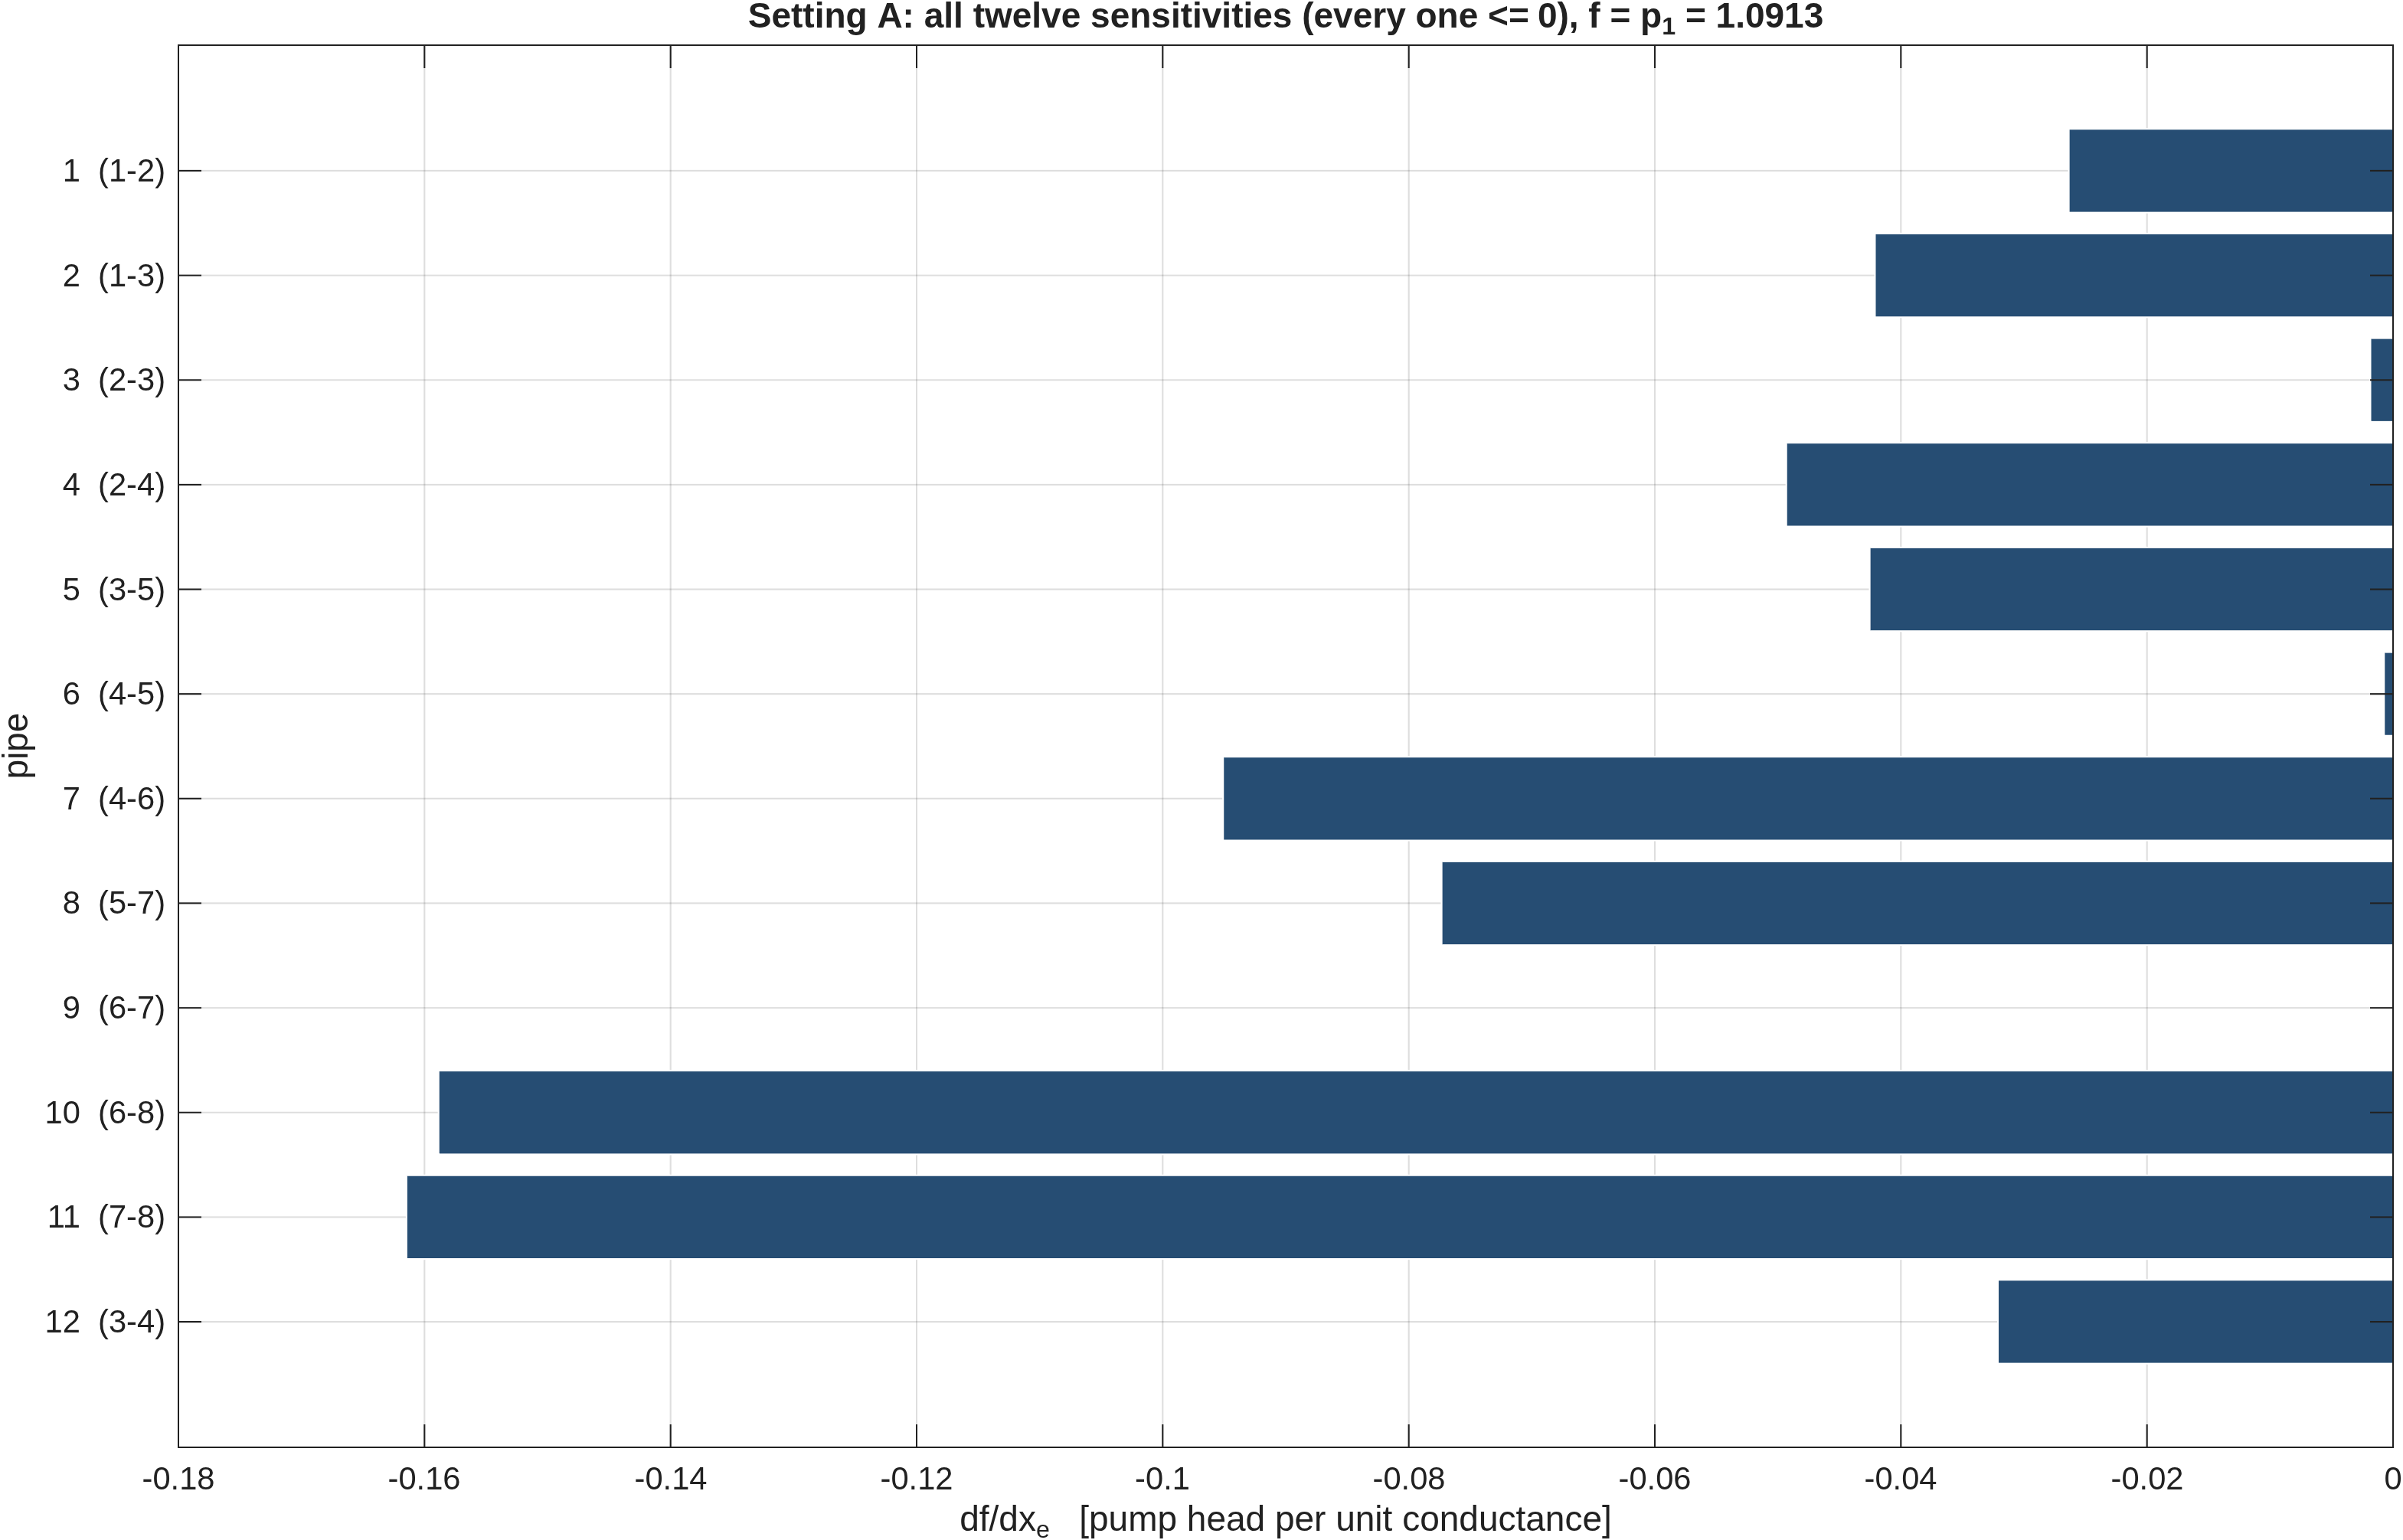
\includegraphics[width=0.66\linewidth]{a3_q1_sensitivities.png}
\caption{The twelve sensitivities of Setting A: every one negative, the two outlet
pipes dominant.}
\end{figure}

\section*{Question 2: Truss size optimisation --- the Michell cantilever}

Scripts: \texttt{a3\_q2\_truss\_sizeOpt.m} (the Lecture 6 demo with the
boundary-condition block replaced) and \texttt{a3\_q2\_parameter\_study.m} (the
three runs of 2.2). The supports are specified physically and snapped to the
nearest left-edge node, so the same code works on both grids:

\begin{quote}\small\ttfamily
leftNodes = find(abs(nodalCoordinates(:,2)) < 1e-12);\\
supportHeight = [Ly/4; 3*Ly/4];\\
{[}\textasciitilde, nearest{]} = min(abs(nodalCoordinates(leftNodes,3) - supportHeight(k)));
\end{quote}

At $h_y = 1$~m and $0.5$~m both snaps are exact. The load node is found the same
way, at $(L_x, L_y/2) = (6,2)$.

\subsection*{2.1 Getting it running}

\begin{center}
\begin{tabular}{rlp{8.3cm}}
\toprule
 & value & comment \\
\midrule
1. fixed DOFs        & 4 of 70 & two pinned points $\times$ two directions --- correct, since only two \emph{points} are pinned, not the edge. Three is the minimum needed to remove two translations and a rotation. \\
2. exit flag         & 1 & first-order optimality and feasibility met to tolerance: \texttt{firstorderopt} $=9.0264\times10^{-7}$ against $10^{-6}$. \\
3. iterations        & 1677 & of 5000 allowed, 1681 function evaluations --- not an iteration limit \\
4. $f_0$             & $1.150128\times10^{3}$ J & uniform start \\
\phantom{4.} $f^\star$ & $1.824175\times10^{2}$ J & \\
\phantom{4.} $f^\star/f_0$ & 0.158606 & the same steel, rearranged, is $6.3\times$ stiffer \\
5. volume, physical  & $1.999997\times10^{-1}$ m$^3$ & of $V = 0.2$ \\
\phantom{5.} normalised & 0.999998 & tight to $-1.6\times10^{-6}$ \\
6. \texttt{lambda.ineqlin} & $1.587548\times10^{-1}$ & $>0$, so the budget is active --- as it must be, since $\partial f/\partial A_e \le 0$ means nothing in the objective stops the optimiser thickening every bar \\
7. bars above 1\%    & 38 of 386 & 348 removed; the line sits at $a = 8.774\times10^{-5}$ m$^2$ and the surviving 38 hold 99.8\% of the volume \\
\bottomrule
\end{tabular}
\end{center}

A sizing problem with fixed nodes has chosen a \emph{topology}, by driving 90\% of
the bars onto their lower bound. $A_{\min}$ is $10^{-7}$ rather than zero so that
$\bm{K}$ cannot go singular.

\begin{figure}[htbp]
\centering
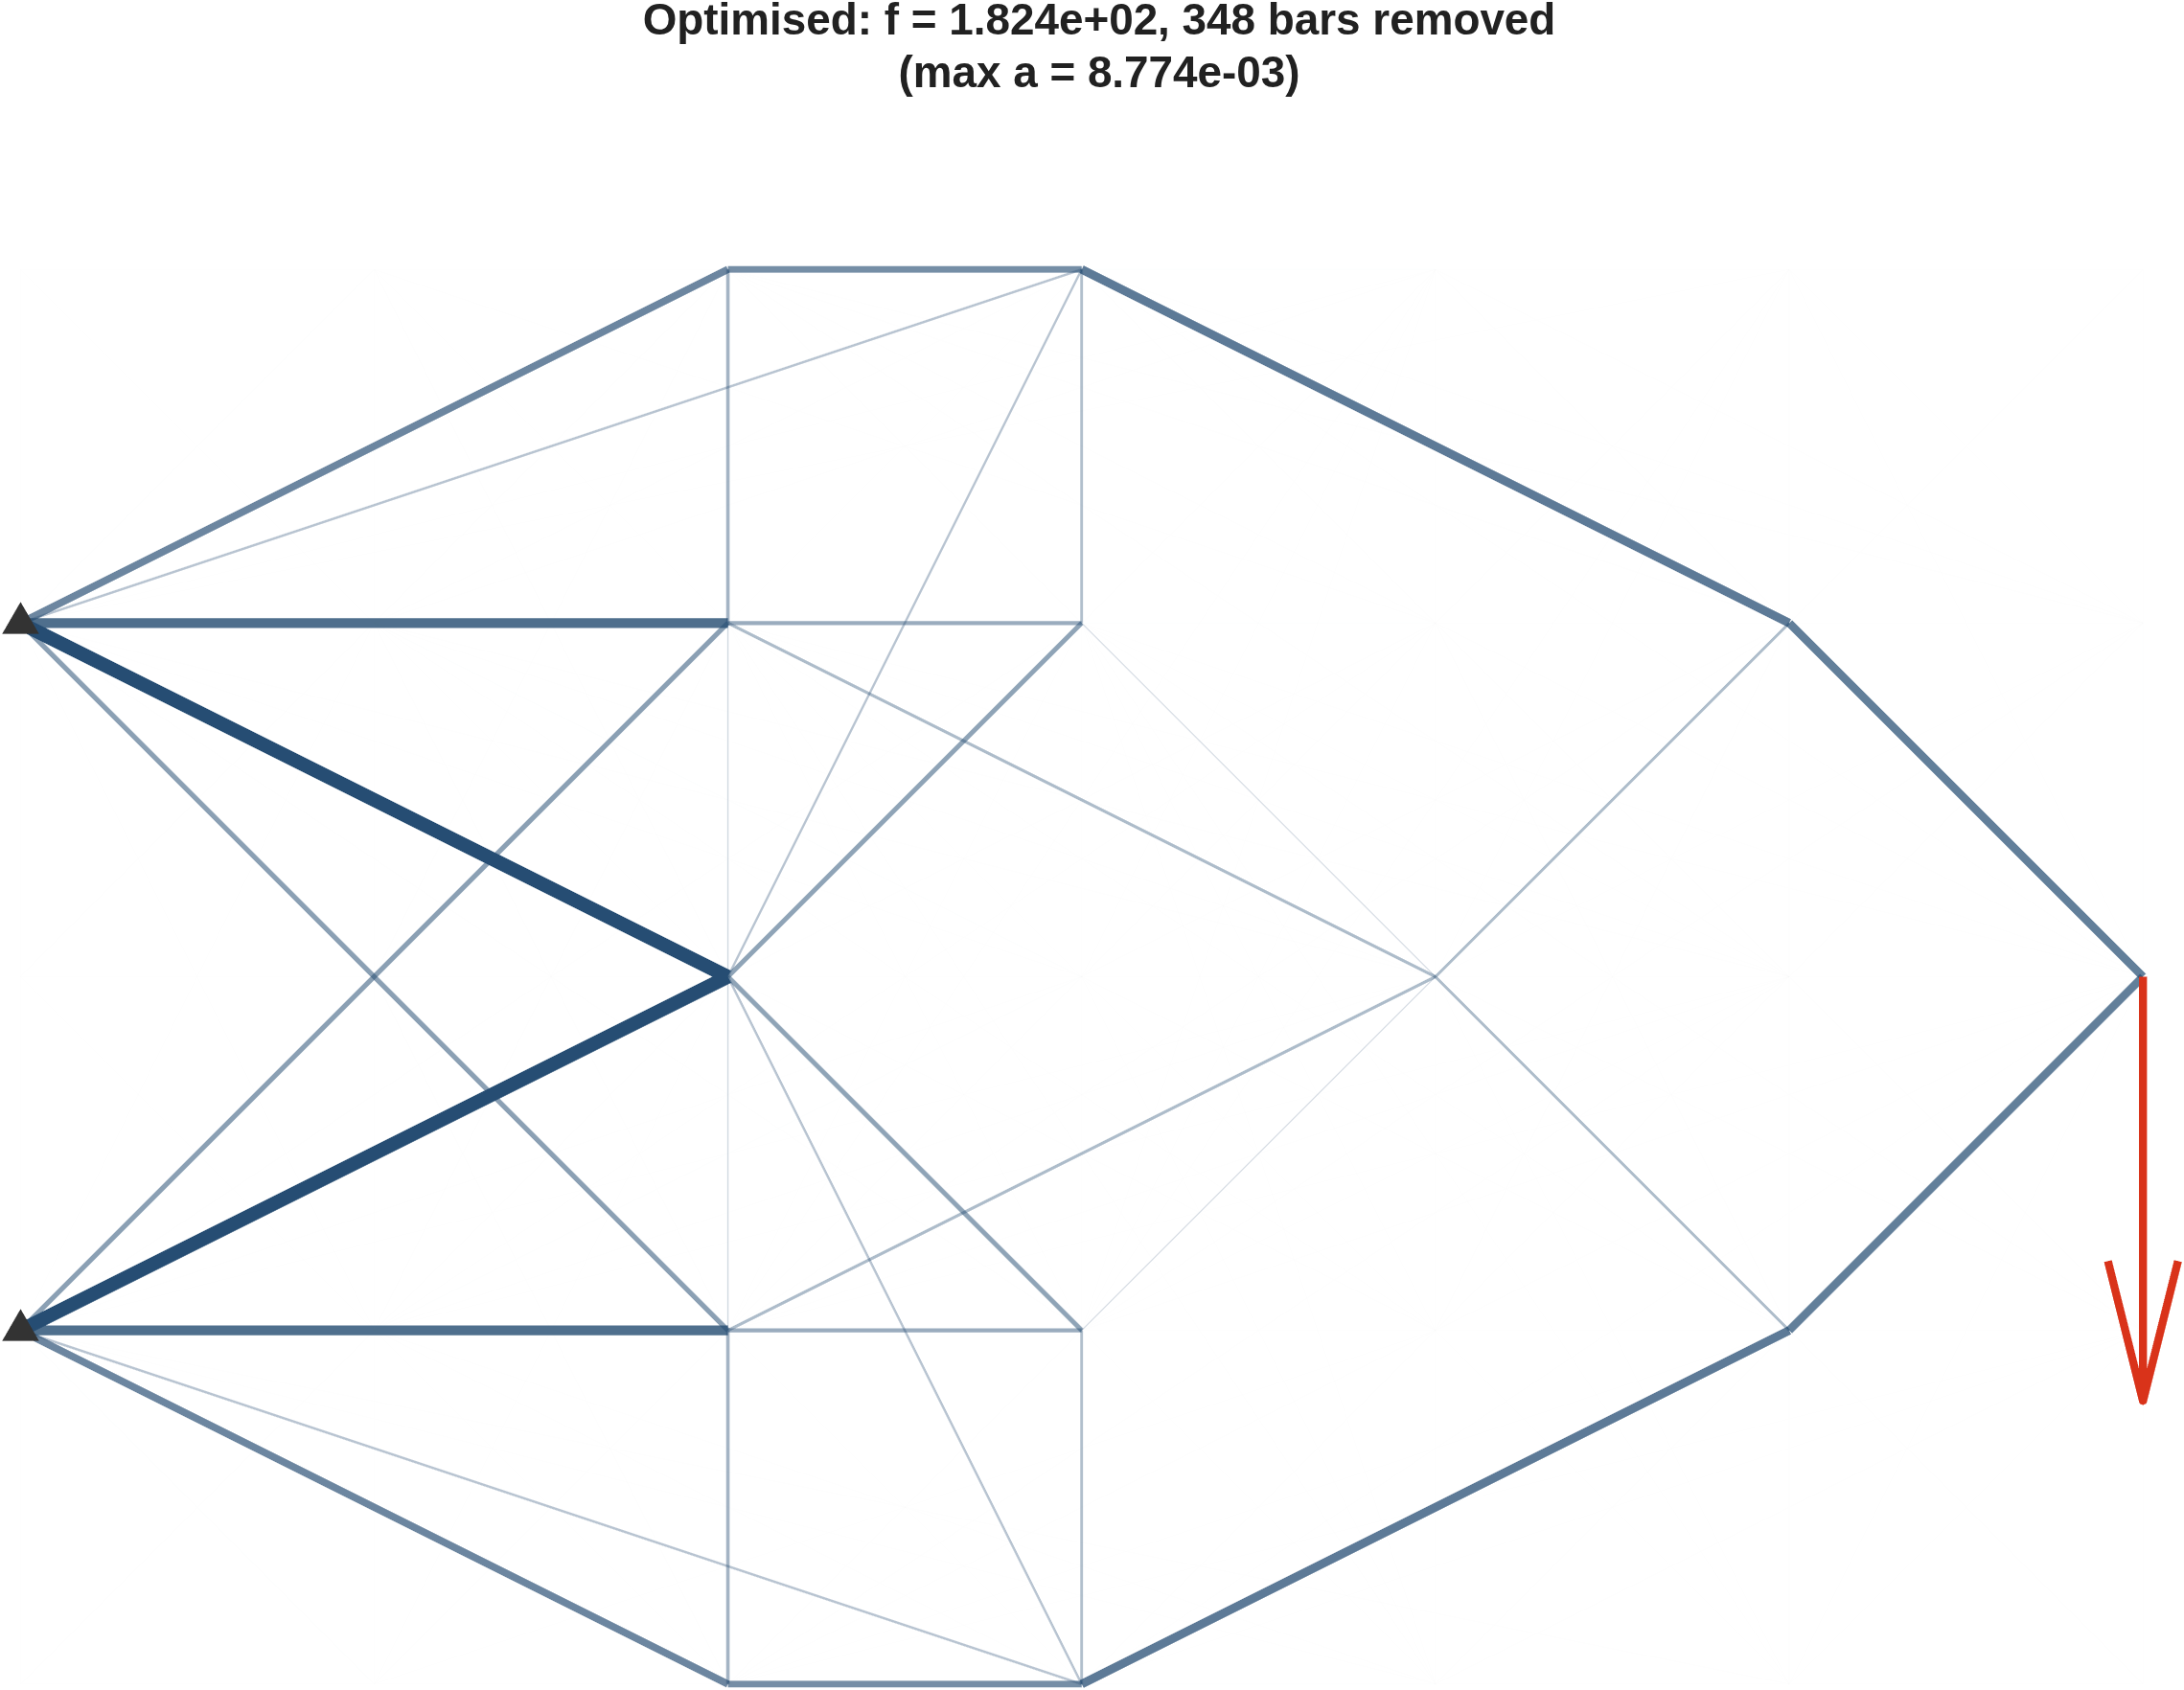
\includegraphics[width=0.70\linewidth]{a3_q2_structure_7x5_full.png}
\caption{Item 8: the optimised baseline --- a tapered lens, deep at the supports
and narrowing to the load, with members fanning at both ends: a Michell
cantilever.}
\end{figure}

\begin{figure}[htbp]
\centering
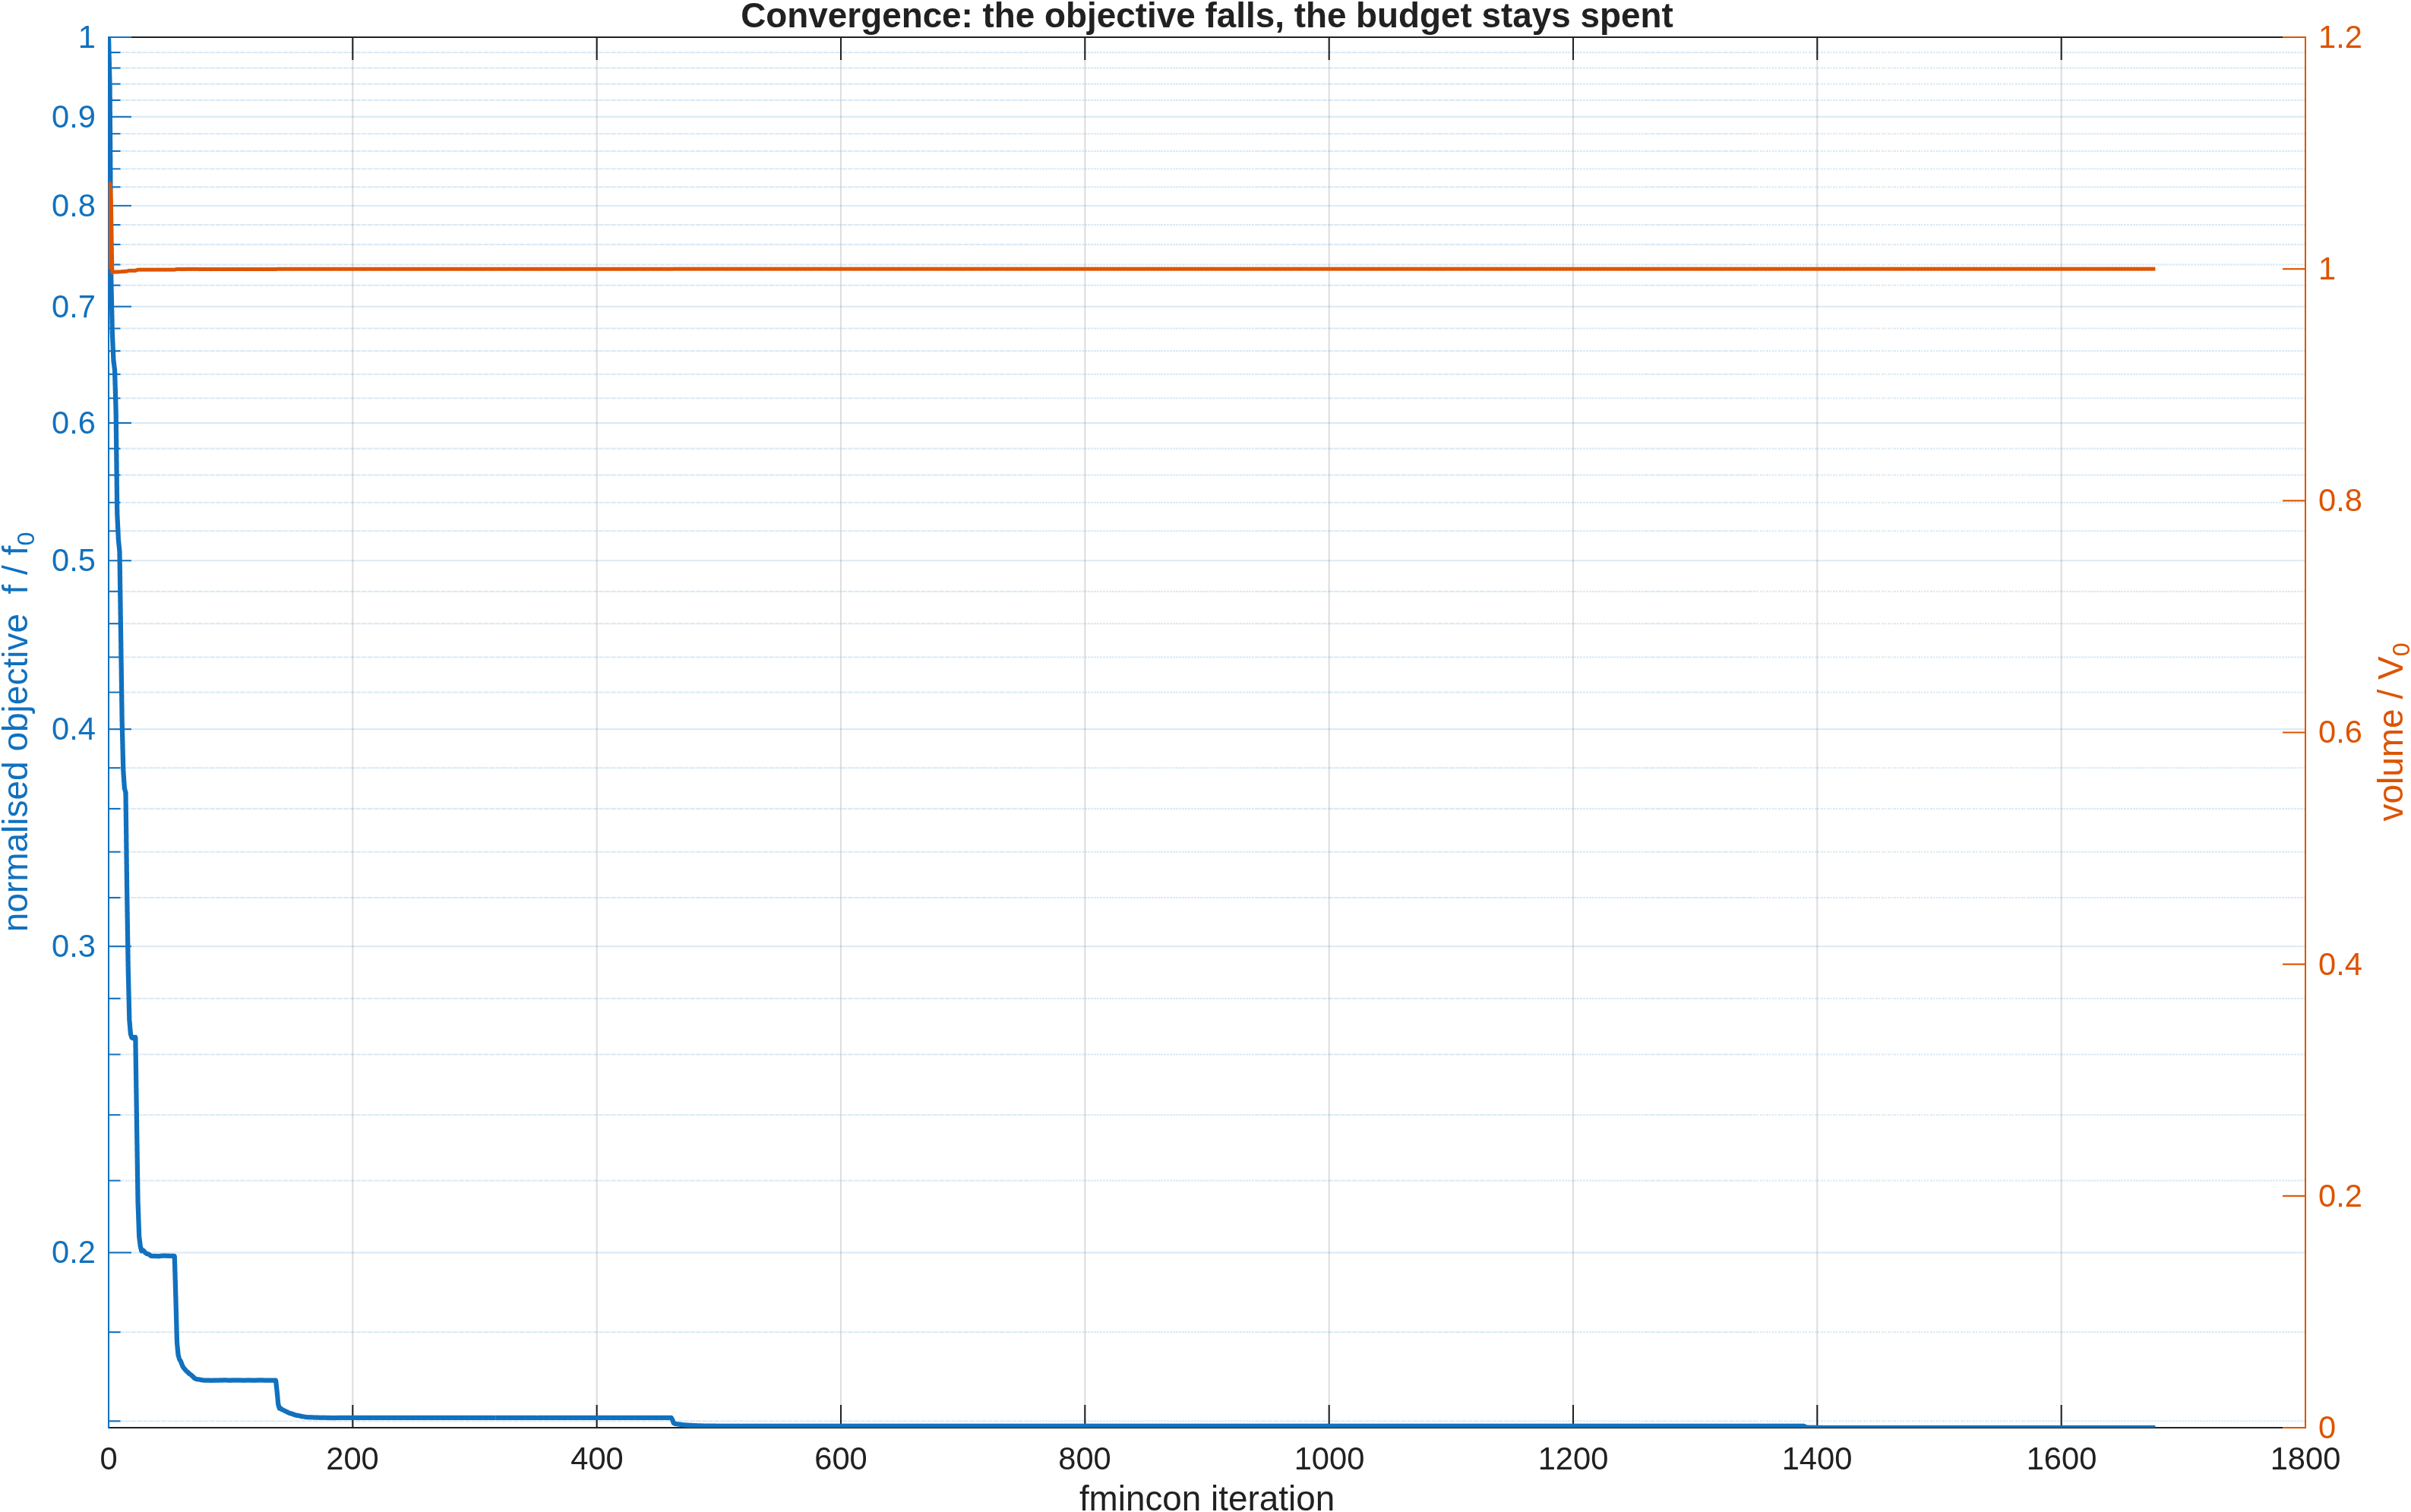
\includegraphics[width=0.70\linewidth]{a3_q2_convergence_7x5_full.png}
\caption{Item 8: convergence. $f/f_0$ falls from 1 to 0.1586; the budget is pinned
at 1 throughout. The staircase is the interior-point barrier parameter being cut
--- a plateau is one subproblem converging, not convergence, which is why the exit
flag is read before the curve.}
\end{figure}

\begin{figure}[htbp]
\centering
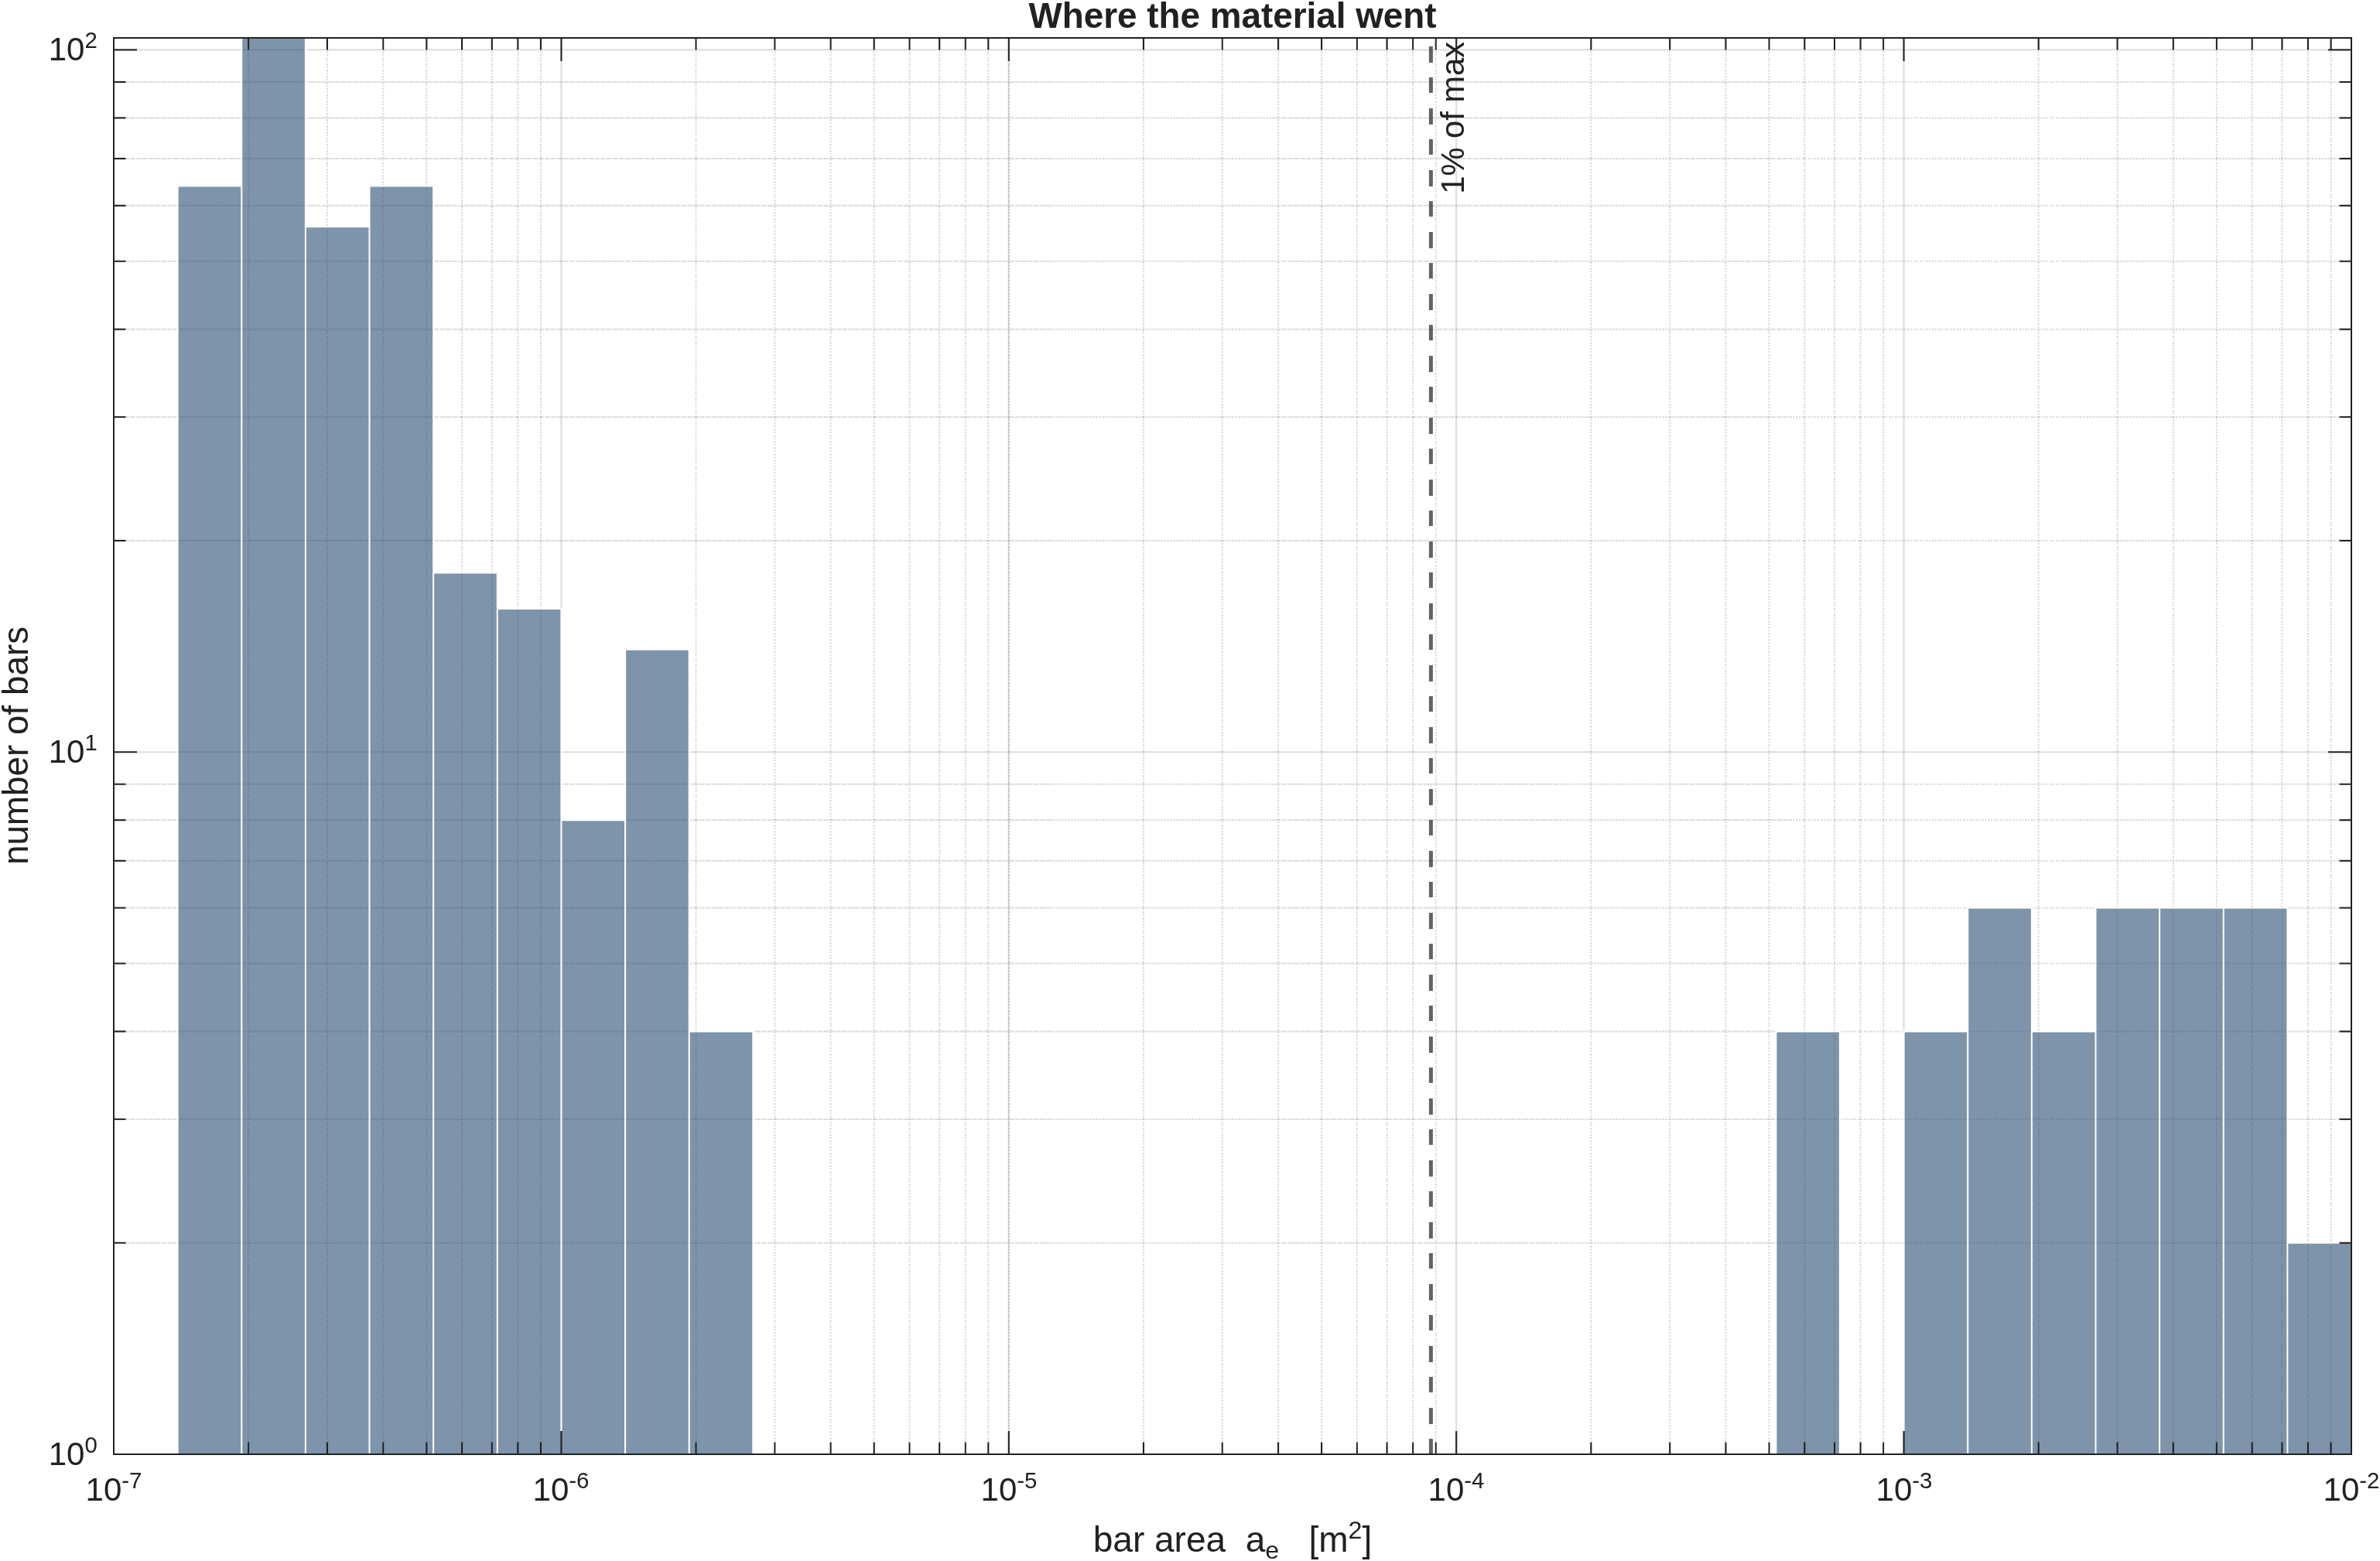
\includegraphics[width=0.70\linewidth]{a3_q2_histogram_7x5_full.png}
\caption{Item 8: the area histogram, log axis, with the 1\% line. Bimodal --- a
crowd at $A_{\min}$ and a few thick bars, little between. The optimiser discards
bars rather than thinning them.}
\end{figure}

\subsection*{2.2 Parameter studies}

\begin{figure}[htbp]
\centering
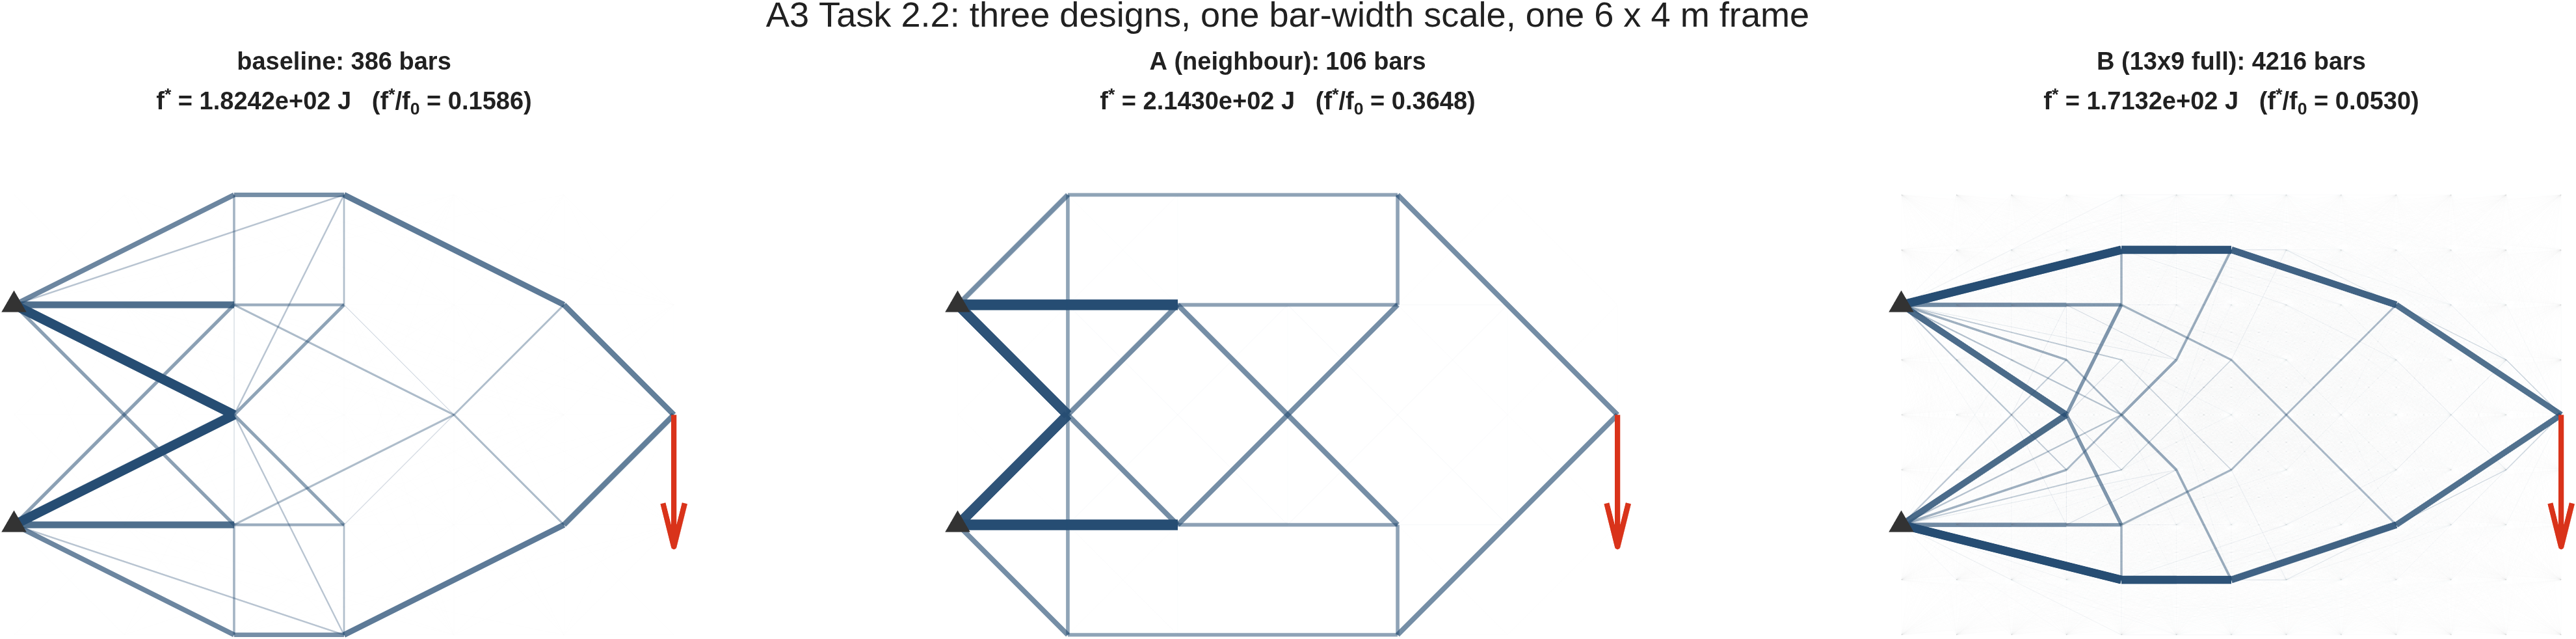
\includegraphics[width=\linewidth]{a3_q2_three_designs.png}
\caption{Item 1: the three optimised designs, same bar-width scale, axes fixed to
the full $L_x \times L_y$ domain in every panel.}
\end{figure}

\textbf{(2) The comparison.}

\begin{center}
\small\setlength{\tabcolsep}{3.4pt}
\begin{tabular}{llrrrrrr}
\toprule
run & setting & bars & $f_0$ [J] & $f^\star$ [J] & $f^\star/f_0$ & $>1\%$ & $\lambda$ \\
\midrule
baseline & $(7,5)$, full      & 386  & $1.150128\times10^{3}$ & $1.824175\times10^{2}$ & 0.15861 & 38 & $1.587548\times10^{-1}$ \\
A        & $(7,5)$, neigh. & 106  & $5.874909\times10^{2}$ & $2.143026\times10^{2}$ & 0.36478 & 34 & $3.635786\times10^{-1}$ \\
B        & $(13,9)$, full     & 4216 & $3.233585\times10^{3}$ & $1.713217\times10^{2}$ & 0.05298 & 90 & $5.426695\times10^{-2}$ \\
\bottomrule
\end{tabular}
\end{center}

$f_0$ differs by run because the same budget is spread over different total bar
lengths, so $f^\star/f_0$ and $\lambda$ are \emph{within-run} quantities. Only
$f^\star$ compares across runs.

\textbf{(3) Run A --- connectivity.} The \textbf{baseline} is lower,
$1.8242\times10^{2}$ against $2.1430\times10^{2}$, by 14.9\%. It must be: every
'neighbour' design is also a 'full' design with the long diagonals left at
$A_{\min}$, so 'neighbour''s feasible set is a \emph{subset} of 'full''s, and a
minimum over a subset cannot be lower. The gap is visible in the figure ---
'neighbour' has only horizontal, vertical and $45^\circ$ members, so it
approximates the diagonal load path in steps. \textbf{We pay} 386 bars against
106 and 4.96~s against 0.80~s.

\textbf{(4) Run B --- refinement.} \textbf{B} is lower, $1.7132\times10^{2}$
against $1.8242\times10^{2}$, by 6.1\%. It must be, because the grids
\emph{nest}: halving both spacings keeps every coarse node. A coarse bar is not
itself a candidate in the fine structure --- the 'full' rule drops any bar with a
third node on it --- but two collinear fine bars of length $L/2$ and area $A$ in
series have stiffness $EA/L$ and volume $LA$, exactly the coarse bar. So the
coarse feasible set embeds in the fine one and $f^\star$ must fall. (Refinement
alone does not guarantee this: the lecture's $11\times5 \to 13\times5$ raises
$f^\star$ from $2.220\times10^{2}$ to $2.302\times10^{2}$ because those grids do
not nest.) \textbf{Cost:} 4216 bars against 386 ($10.9\times$) and 78.2~s against
4.96~s ($15.8\times$), for 6.1\%. \textbf{Would we pay it?} For a final design
yes --- 6\% is free stiffness bought once. Inside a loop, no. The trend decides:
the baseline captured 14.9\% over A, B added a diminishing 6.1\% at sixteen times
the cost, so the next halving is not worth running.

\section*{Declaration of AI use}

We used an AI assistant (Claude, Anthropic) while preparing this hand-in. What
we used it for:

\begin{enumerate}\itemsep0pt
\item \textbf{English.} Correcting grammar and rephrasing passages so that they
      read more clearly. What each rephrased sentence says is ours; the wording
      was improved.
\item \textbf{Typesetting the mathematics.} Writing the equations of this report
      in \LaTeX{} --- turning mathematics we had already worked out into typeset
      form.
\item \textbf{Fixing \LaTeX{}.} Diagnosing compilation errors and correcting
      formatting problems: misaligned tables, figure placement and spacing.
\item \textbf{Explaining code.} Explaining parts of the MATLAB used in this
      assignment. \textbf{[TO BE COMPLETED: name the specific functions and
      scripts this covers.]}
\end{enumerate}

Every number in this report was produced by our own scripts and read from their
printed output, and every claim above is one we can derive and defend.

\end{document}
